\index{general}{Lyapunov Time}

%from wiki

Simply put, the Lyapunov time is the characteristic timescale on which a dynamical system is chaotic.
 It is defined as the inverse of a system's largest Lyapunov exponent.

The Lyapunov time mirrors the limits of the predictability of the system. By convention, it is defined 
as the time for the distance between nearby trajectories of the system to increase by a factor of $e$. 
However, measures in terms of 2-foldings and 10-foldings are sometimes found, since they correspond to 
the loss of one bit of information or one digit of precision respectively.

The Lyapunov exponent or Lyapunov characteristic exponent of a dynamical system is a quantity 
that characterizes the rate of separation of infinitesimally close trajectories. 
Quantitatively, two trajectories in phase space with initial separation $\delta \mathbf{Z}_0$ 
diverge (provided that the divergence can be treated within the linearized approximation) at a rate given by
\[
|\delta \mathbf{Z} (t)|\approx e^{\lambda t}|\delta \mathbf {Z} _{0}| 
\]
where $\lambda$ is the Lyapunov exponent. 

Measuring the Lyapunov exponent or time (or related quantities) is relevant in the context of mantle stirring. 
On the one hand it is argued that the mantle is convecting and very efficient at mixing resulting in a 
somewhat homogenous composition. On the other hand, there is are modeling studies that suggest that
whole-mantle convection can preserve heterogeneity in the presence of well-mixed mantle. 

%from vazh99
Mixing takes place by the repeated stretching
and folding of interfaces. A measure of the
mixing efficiency is the time evolution of the area of
the mixing surface. Maximum efficiency of mixing
is reached with turbulent mixing behavior where
One can formally show whether mixing is laminar or turbulent by evaluating the Luyaponov exponents $\sigma$ .
These are of the form:
\[
\sigma = \lim_{t\rightarrow \infty} \lim_{X\rightarrow 0} \left[  \frac{1}{t} \ln \left( \frac{X(t)}{X(t=0)} \right)   \right]
\]
where $X(t)$ is the length of this segment at time t.
Non-zero Luyaponov exponents indicate that
stretching is exponential and the larger the exponent,
the more efficient mixing is.
However, the limits in the above equation are difficult to evaluate and the interpretation 
of the 'finite-time' Luyaponov exponent, where both limits are truncated, is difficult to formalize.


Two approaches are taken in the literature when it comes to studying mixing/stirring and/or measuring Lyapunov quantities::

\begin{itemize}
\item using marker advection: in van Keken and Zhong \cite{vazh99} the authors use a steady state velocity
pattern obtained for a model of present-day mantle convection. The velocity model is
based on the solution of the Stokes equations in a 3D spherical model with variable rheology.
To study mixing, they release particles in the velocity model and follow 
these by numerical integration. 

\begin{center}
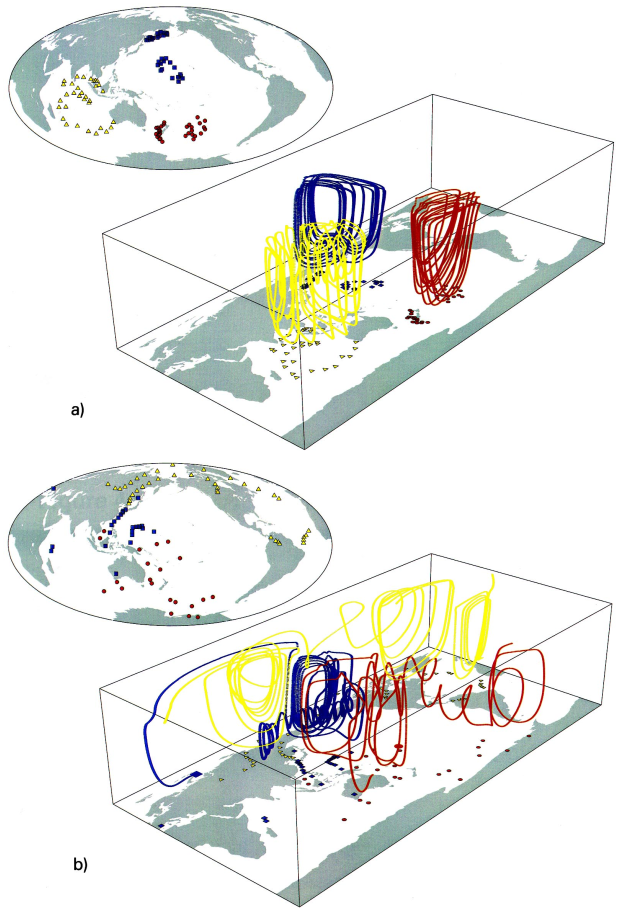
\includegraphics[width=7cm]{images/mixing/vazh99}\\
{\captionfont a) The three particles in this plot were
selected for their relatively regular pattern. 
b) Three other particles that traverse a large portion of the model. These particles feel 
the strong toroidal motion and their paths form corkscrew-like patterns. 
They indicate that certain parts of the model can exhibit strong mixing.  Taken from \cite{vazh99}.}
\end{center}

Rather than calculating the exponents explicitly, the authors 
use an approximation to the finite-time,
finite-length Luyaponov exponent by evaluating the distance between two points that are closely spaced
at time $t=0$. For this they compute the advection of a
large number of 10 km long line segments that were
originally at 1500 km depth. The length of these segments is approximated by the distance between the
endpoints and the results are summarized in the following figure:

\begin{center}
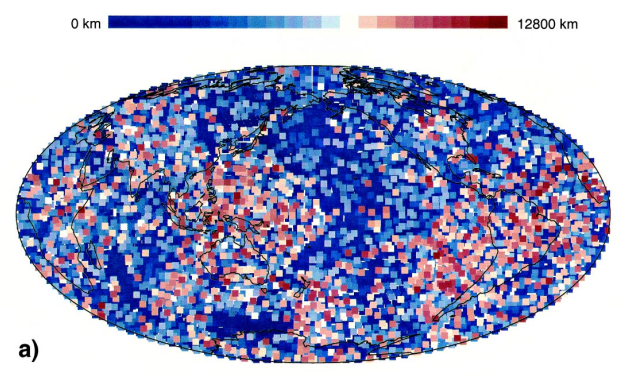
\includegraphics[width=7cm]{images/mixing/vazh99b}\\
{\captionfont Length
of the line segment after 4 billion years. Approximately 14,000 line segments were released with 
regular spacing at 1500 km depth. The length of the segment is indicated by the colored symbols 
that are plotted at the initial position. The results indicate that there is a strong
diversity in mixing behavior. In some regions (north Pacific, parts under the Indian/Australian plate) 
stretching is very limited, indicating laminar and consequently inefficient mixing. Regions that 
are under strong toroidal surface motion (western Pacific, Nazca and South
America) show very efficient stretching of up to the maximum length of the diameter of the Earth. 
Taken from  \cite{vazh99}.}
\end{center}



\item twin experiments \cite{becr14}
\end{itemize}


Talk about configurational entropy \cite{gobo02,nake07}.

Talk about retrodiction \cite{cobs15,cogb18}

\Literature \cite{vazh99,falt02,fasa03,saad11,sato12,becr14,cobs15}

